\documentclass{article}
\usepackage{amsmath,amsthm,amssymb}
\usepackage{mathtext}
\usepackage[T2A]{fontenc}
\usepackage[utf8]{inputenc}
\usepackage[russian]{babel}
\usepackage{graphicx}
\usepackage{hyperref}

\title{Построение эмбеддингов крымскотатарских слов: корпус, модели, валидация}
\author{Пеганов Никита}
\date{июнь 2025}

\begin{document}
\maketitle
\begin{abstract}
    В работе описан процесс построения корпуса текстов на крымскотатарском языке, очистки, лемматизации и создания семантических эмбеддингов (CBOW и SVD). Ключевая особенность — подробная валидация каждого шага с носителями языка с целью минимизации шума и смешанных слов. Отдельное внимание уделено успешному применению локальной LLM DeepSeek для фильтрации лексики. Ссылка на репозиторий: \url{https://github.com/NikPeg/qt-embeddings}
\end{abstract}

\section{Введение}
Обработка текстов на языках с низкими ресурсами (например, крымскотатарском) сталкивается с отсутствием инструментов, нечистыми корпусами, смешанным письмом и нехваткой лингвистических ресурсов. Семантические эмбеддинги для такого языка крайне важны: они позволяют автоматизировать задачи классификации, морфоанализа, машинного перевода, а также лингвистических исследований языков народов России.

Особенность нашего проекта — на каждом этапе обработки данные проверялись носителями крымскотатарского языка, чтобы исключить шум, ошибки, заимствования и обеспечить чистоту корпуса. Мы также применили современные нейросетевые инструменты (LLM DeepSeek) — и их результаты дополнительно валидировались носителями.

В перспективе планируется существенно увеличить корпус за счёт автоматического сбора (краулинга) с большего числа сайтов и ресурсов.

\subsection{Команда}
\textbf{Пеганов Никита} — единственный участник команды, выполнил сбор, обработку данных, построение моделей и написание отчёта. Все этапы предварительно консультировались с носителями языка.

\section{Связанные работы}
\label{sec:related}
Классические эмбеддинги (Word2Vec CBOW, Skip-Gram~\cite{mikolov2013distributed}, FastText~\cite{bojanowski2017enriching}) хорошо работают для ресурсных языков, но не применяются напрямую к крымскотатарскому из-за морфологических и орфографических особенностей, шума и смешения с другими языками.

Турецкий лемматизатор Zeyrek~\cite{zeyreklem} был протестирован, но показал низкое качество — высокая доля ошибок из-за различий крымскотатарского и турецкого.
Применение локальных LLM (например, DeepSeek~\cite{deepseek2024}) с несколькими вариациями промпта дало высокую точность фильтрации лексики, но требует обязательной ручной валидации носителем.

\section{Описание модели}
Конвейер обработки представлен на рис.~\ref{fig:flowchart} и включает следующие этапы:

\textbf{1. Сбор данных:}
Открытые крымскотатарские тексты из интернета, книг, СМИ.

\textbf{2. Очистка и токенизация:}
Удаление мета-текста, нормализация орфографии и пунктуации, фильтрация русских/турецких и других фрагментов, разбиение на предложения и токены.

\textbf{3. Лемматизация:}
Собственный гибридный лемматизатор: словарь + эвристики для морфологии, сравнение с турецким и LLM-инструментами, ручное подтверждение чистоты.

\textbf{4. Минимизация шума:}
На каждом этапе результаты сверялись с носителями языка — это многократно уменьшило количество "мусорных" и лишних слов.

\textbf{5. Применение LLM (DeepSeek):}
Был развёрнут локальный LLM DeepSeek-R1-Distill-Qwen-32B, к которой применялись различные промпты для определения, является ли слово крымскотатарским. Классификация неоднозначных лексем проводилась с несколькими проходами; итоговые списки подтверждал носитель.

\textbf{6. Построение эмбеддингов:}
Тренировка эмбеддингов CBOW (gensim), дополнительно — SVD по матрице совместных появлений.

\begin{figure}[!tbh]
    \centering
    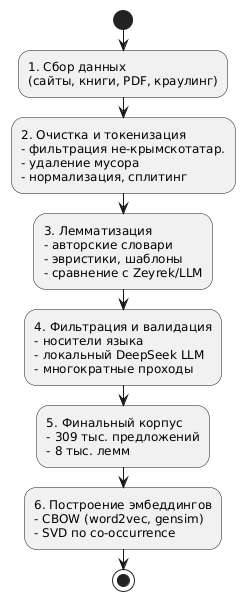
\includegraphics[width=0.85\linewidth]{pipeline.png}
    \caption{Схема обработки корпуса и построения эмбеддингов.}
    \label{fig:flowchart}
\end{figure}

\section{Корпус данных}

Датасет для обучения был собран на основе открытых источников: крымскотатарских сайтов, электронных книг, газет и архивов СМИ. Детализированная статистика по количеству документов, предложений и токенов приведена в таблице~\ref{tab:statistics}.

Для автоматизации сбора был разработан и использован отдельный пакет краулеров, исходный код которого доступен по ссылке: \url{https://github.com/NikPeg/qirimtatar-embedding-crawlers}. С помощью этого инструмента были загружены и предобработаны данные из различных интернет-источников — от литературы до современных публикаций. Краулеры поддерживают не только парсинг html-страниц, но и обработку документов в форматах DOC, PDF, а также распознавание текстов с изображений при помощи Tesseract OCR. Особое внимание уделялось корректному определению крымскотатарского языка (через Яндекс API) и фильтрации нерелевантных материалов (например, обучение, материалы на русском языке и пр.).

Парсер содержит многопоточные модули для быстрой выгрузки архивов, систему удаления нежелательных водяных знаков (Aspose), а также полноценный конвертер изображений и PDF в текстовый формат с учётом особенностей обработки крымскотатарского письма.

Процесс сбора и предобработки включал:
\begin{itemize}
    \item автоматизированный сбор текстов с различных источников (сайты, гугл-документы, архивы и пр.);
    \item извлечение текста из PDF, DOC и изображений (OCR);
    \item фильтрацию языковых артефактов и удаление мусорных файлов;
    \item определение языка каждого фрагмента с помощью Яндекс API;
    \item удаление учебных текстов и материалов на других языках на основе стоп-слов и ручной проверки.
\end{itemize}

Итоговые наборы документов (более 10 ГБ в сжатом виде) доступны для скачивания по ссылкам, приведённым в README краулер-репозитория (Яндекс.Диск, HTTP, FTP по запросу).

Очищаются:
\begin{itemize}
    \item Русские, турецкие и любые не-qt-фрагменты
    \item Нормализация орфографии, пунктуации
    \item Разметка предложений, токенизация
    \item Лемматизация и фильтрация — всё валидировано носителями языка
\end{itemize}

Обработано $\sim$309 тыс. предложений и более 3 млн токенов, извлечено 8245 лемм.

\begin{table}[tbh!]
\begin{center}
\begin{tabular}[t]{|l|c|}
\hline
 & Значение \\
\hline
Файлов & 123  \\
Предложений & 309,334 \\
Токенов & 3,157,286 \\
Лемм & 8,245 \\
Оценка OoV & $<$5\% (после очистки) \\
\hline
\end{tabular}
\caption{Статистика корпуса крымскотатарских текстов. После финальной фильтрации доля "мусора" минимальна.}
\label{tab:statistics}
\end{center}
\end{table}

\textbf{Будущая работа:} в перспективе планируется существенное увеличение корпуса за счёт автоматического сбора текстов с сайтов и форумов.

\section{Эксперименты}
\subsection{Метрики}
Для оценки применялись:
\begin{itemize}
    \item Доля корректно лемматизированных и распознанных токенов (по оценке носителей)
    \item Семантическая связность соседей в эмбеддингах (ручная проверка)
    \item Сравнение OoV после разных фильтров: Zeyrek, DeepSeek и примитивный baseline
\end{itemize}

\subsection{Экспериментальная настройка}
Проводилось:
\begin{itemize}
    \item Сравнение разных подходов к лемматизации/фильтрации: свой, Zeyrek, DeepSeek
    \item Тренировка CBOW-эмбеддингов (50 эпох, размер вектора 100, окно 5, мин.частота 3), SVD-эмбеддингов (100 компонент)
    \item Весь результат этапов валидировался носителями языка — особое внимание к самым частотным словам
\end{itemize}

\subsection{Бейслайны}
Использовались:
\begin{itemize}
    \item Примитивная лемматизация и фильтрация
    \item Турецкий лемматизатор Zeyrek
    \item LLM DeepSeek для языковой фильтрации
    \item Случайный/частотный baseline для анализа ошибок
\end{itemize}

\section{Результаты}
\textbf{Чистота корпуса:} Валидация на всех этапах сильно снизила шум и количество не-крымскотатарских слов. Правила+словари дали покрытие 25.5\% по леммам, Zeyrek — только 2.8\%. Осталось $\approx$14 тыс. нерспознанных токенов (vs 27 тыс. у Zeyrek).

\textbf{Собственный лемматизатор:} В процессе построения корпуса был разработан специализированный лемматизатор, основанный на расширенной версии турецкого лемматизатора Zeyrek c добавлением крымскотатарских словарей, правил и морфологических шаблонов. Данная система показала значительно лучшие результаты по сравнению с турецкой версией и может быть использована как самостоятельный инструмент для обработки текстов на крымскотатарском языке в будущих исследовательских и прикладных задачах.

\textbf{LLM-фильтрация:} Локальный DeepSeek с несколькими итерациями промпта показал отличную точность в фильтрации не-qt-лексики; все сомнительные случаи рассматривались с носителем.

\textbf{Эмбеддинги:} CBOW и SVD хорошо группируют семантически близкие слова (см. табл.~\ref{tab:neighbors}).

\begin{table}[!tbh]
    \centering
    \begin{tabular}{|l|l|l|l|l|l|}
\hline
\textbf{Запрос} & \textbf{1} & \textbf{2} & \textbf{3} & \textbf{4} & \textbf{5} \\
\hline
\texttt{халкъ}  & феодализм & adam & дюль & adalarında & джеси \\
(народ) & (феодализм) & (человек) & (сердце/разум)\footnotemark[1] & (на островах) & (его/её часть)\footnotemark[2] \\
\hline
\texttt{джан}   & ешерди & гоньдже & огюндекиси & узьди & сёзлерининъ \\
(душа) & (прятал(а)) & (юная девушка) & (тот самый) & (оторвал(а)) & (его/её слова) \\
\hline
\texttt{мектеп} & мудири & бетине & эмизе & айда & тaze \\
(школа) & (директор) & (на лицо) & (мать) & (месяц) & (новый, свежий) \\
\hline
\texttt{миллет} & атар & коккозьге & пери & голланд & тенде \\
(нация) & (племя)\footnotemark[3] & (к Коккозу) & (фея) & (Голландия) & (на теле) \\
\hline
\texttt{тиль} & давушнен & менимкини & тааджипленип & суреттс & тюшюндим \\
(язык) & (с голосом) & (мой) & (удивившись) & (изобрази) & (я понял) \\
\hline
    \end{tabular}
    \caption{Ближайшие соседи к частотным словам (CBOW). Переводы приводятся в скобках, "---" — неизвестно.}
    \label{tab:neighbors}
\end{table}

\footnotetext[1]{Значение слова "дюль" требует уточнения, возможно, это форма слова "диля" (сердце, ум).}
\footnotetext[2]{Форма окончания, значение зависит от контекста.}
\footnotetext[3]{В тюркских языках "атар" — "род", "племя" или форма глагола "стрелять".}

\textbf{Качественный вывод:} Семантика сохраняется: например, соседи слова "халкъ" (народ) — слова о сообществе, у "агъыз" (рот) — части тела и речь.

\section{Выводы}
Построен чистый валидированный корпус крымскотатарских текстов, леммы и эмбеддинги (CBOW, SVD). Все этапы были проверены носителями языка — это позволило значительно сократить шум, уменьшить смешение с другими языками. Локально применён LLM DeepSeek для языкового фильтра с несколькими раундами промпта — и подтверждён носителем как рабочий инструмент.

Корпус, эмбеддинги и лемматизированная лексика пригодны для дальнейших NLP, типологических и лингвистических задач для низкоресурсных языков. В перспективе — расширение корпуса за счёт краулинга, проверка эмбеддингов на реальных downstream-задачах, тиражирование инструментов на другие языки народов России.

\bibliographystyle{apalike}
\bibliography{lit}
\end{document}
